\chapter{Improvements in the Analysis}

In the previous chapter, we had show examples where the heap liveness analysis applied to the synchronized control flow graph returned a highly-over approximated access graph. The reason for this being the inter-thread synchronization edges not being treated differently from intra-thread edges. There is also a need to ensure that the final data flow value obtained can actually be a result of valid program execution. \\

In order to achieve this we need to analyze critical sections in all the threads. An intra-thread analysis will be required to be performed. We need to figure out the whether there exists a loop outside the critical section. If there is no such loop then we can say that the critical section will be executed once. Otherwise, The critical section can be executed zero or more times. Note that this information is independent of other threads. Once we have the thread dependent information , we can add inter-thread edges. The edges will only be triggered based on the condition that checks if the critical section can be executed. The condition would involve comparing counters of the number of times a critical section is executed. \\

One way to achieve this is to label the edges with the number of times the transition is possible. Considering the examples in the last chapter figure 5.1, 5.2 and 5.3, we can suggest the following access graphs at the statement main(). See figure 6.1. \\


\begin{figure}
	\centering
	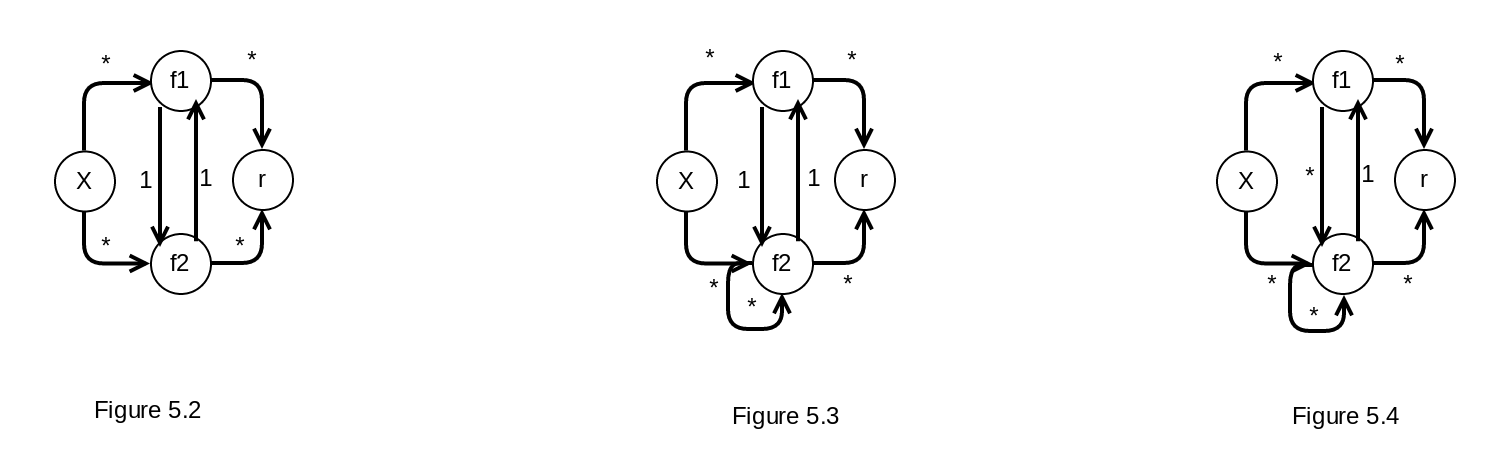
\includegraphics[width=0.8\textwidth]{Figures/access_graph_rep.png}
	\caption{Desired Access graphs for fig 5.2,5.3 and 5.4}
	\label{fig:ch5example}
\end{figure}
 
In examples 5.2,5,3 and 5.4 , we had observed that access graph at the statement main() was the same. We now display the desired representation of access graph. For example 5.2, we have observed that the critical section can only be executed once for both the threads. So we need to mark the edge with either 1 or *, where 1 denotes that the transition can only be performed once and * is a doesn't care condition. \\

For 5.3, we had a loop inside critical section of thread 2. However the critical section could only be executed once. There will be a self loop around $f_2$ in the access graph. The edges from $f_1$ and $f_2$ are representative of a thread change. Since there are no loops across/outside the critical section, we can conclude that both these will execute once and mark the two edges 1. \\

For example 5.4, there is a thread 2 has a loop across the lock and unlock section. Thus now the edge representing transition from $C_1$ to $C_2$ can be executed any number of times. The desired access graph for 5.4, should be the similar to 5.3 except for the edge from $f_1$ to $f_2$ being labeled as * instead of 1. \\

We may need to modify the analysis in order to obtain the desired access graph for all the examples. One way may be to change the way we merge and summarize access graphs different threads.

\section{Concurrent Heap Access examples}

Let us try to understand the how heap memory is actually accessed by threaded programs using shared memory. This will be better understood by taking up the example of a concurrent data structure say tree. Each node of the tree has \emph{l} and \emph{r} fields pointing to children and a \emph{data} field. \\

Consider the simplest example for this, similar to example 5.2 in figure 6.2. The access pattern is either $T_1$ followed by $T_2$ or the reverse. If $T_1$ is executed first then the object \emph{x.l.r} is accessed otherwise \emph{x.r.l} is accessed. This corresponds to the iteration 1 of simple concurrent heap liveness analysis. (See figure 4.4) So if the analysis is stopped at this point we would obtain the desired access graph in this case. \\

\begin{figure}
	\centering
	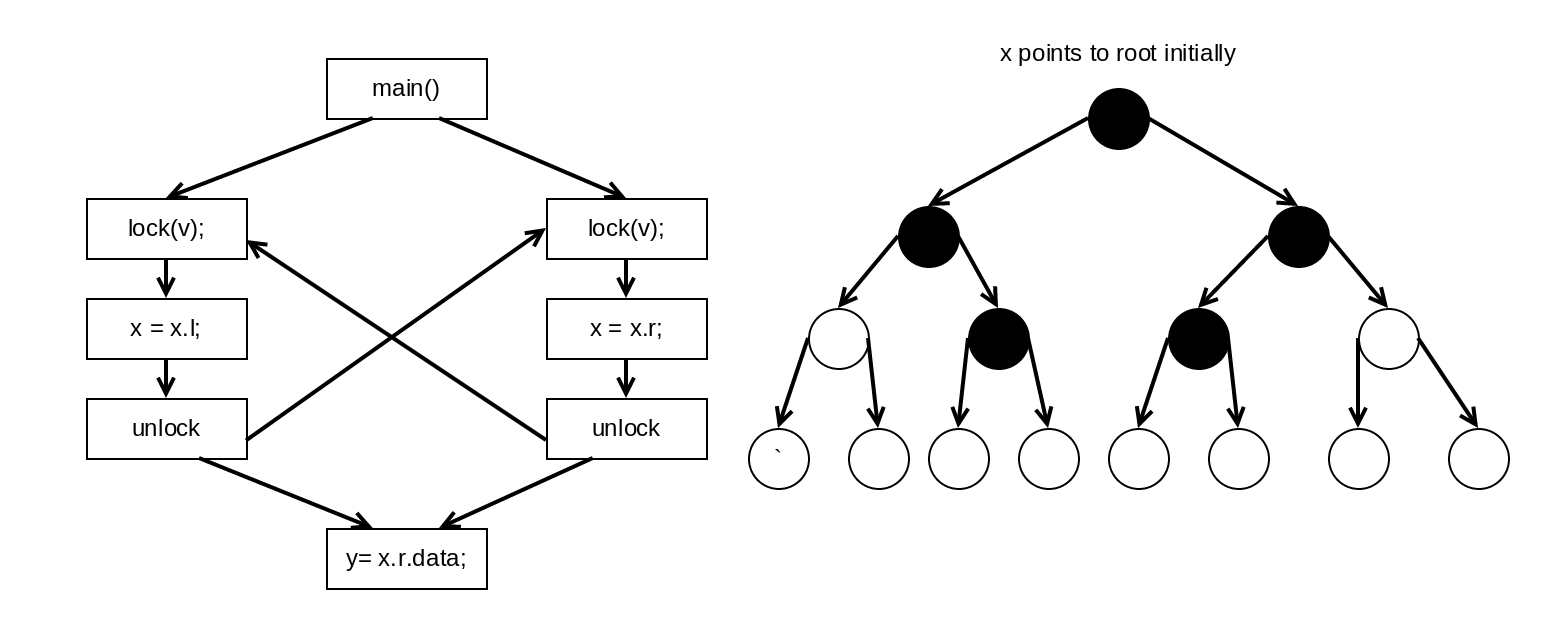
\includegraphics[width=0.8\textwidth]{Figures/tree1.png}
	\caption{Concurrent access example in a tree}
	\label{fig:ch5example}
\end{figure}  

Consider another example with a loop within the critical section in Figure 6.3. This is again inspired from Figure 5.3. Again the access pattern may be either $T_1$ followed by $T_2$ or the reverse. This implies the objects accessed will satisfy the regular expression \emph{x.l.r\textsuperscript{*}} or \emph{x.r\textsuperscript{*}.l} depending on the  starting thread. Figure 6.3 shows the possible nodes that can be accessed by the concurrent program. It just maps the regular expression to the tree topology. \\

\begin{figure}
	\centering
	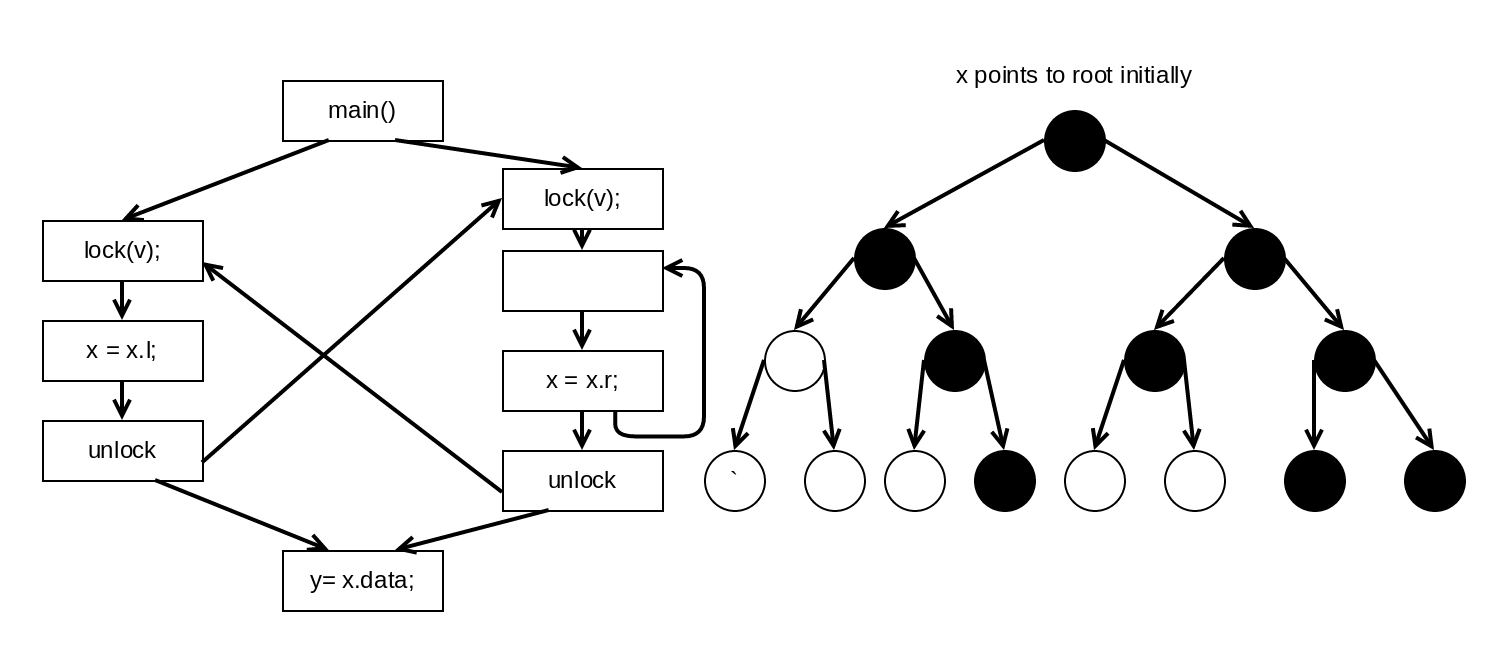
\includegraphics[width=0.8\textwidth]{Figures/tree2.png}
	\caption{Another Concurrent access example in a tree}
	\label{fig:ch5example}
\end{figure}

Now we will look into the possible executions of the example in Figure 6.4. This is the case of presence of loop across critical section. We will have two possible execution orders corresponding to start from $T_1$ or $T_2$ : \emph{x.l.r\textsuperscript{*}}, {x.r\textsuperscript{+}.l.r\textsuperscript{*}}. Looking at the difference between this example and Figure 6.3, we notice that \emph{r\textsuperscript{+}} links from all the nodes of the type \emph{x.r\textsuperscript{+}.l} can be additionally accessed by this program. \\ 

\begin{figure}
	\centering
	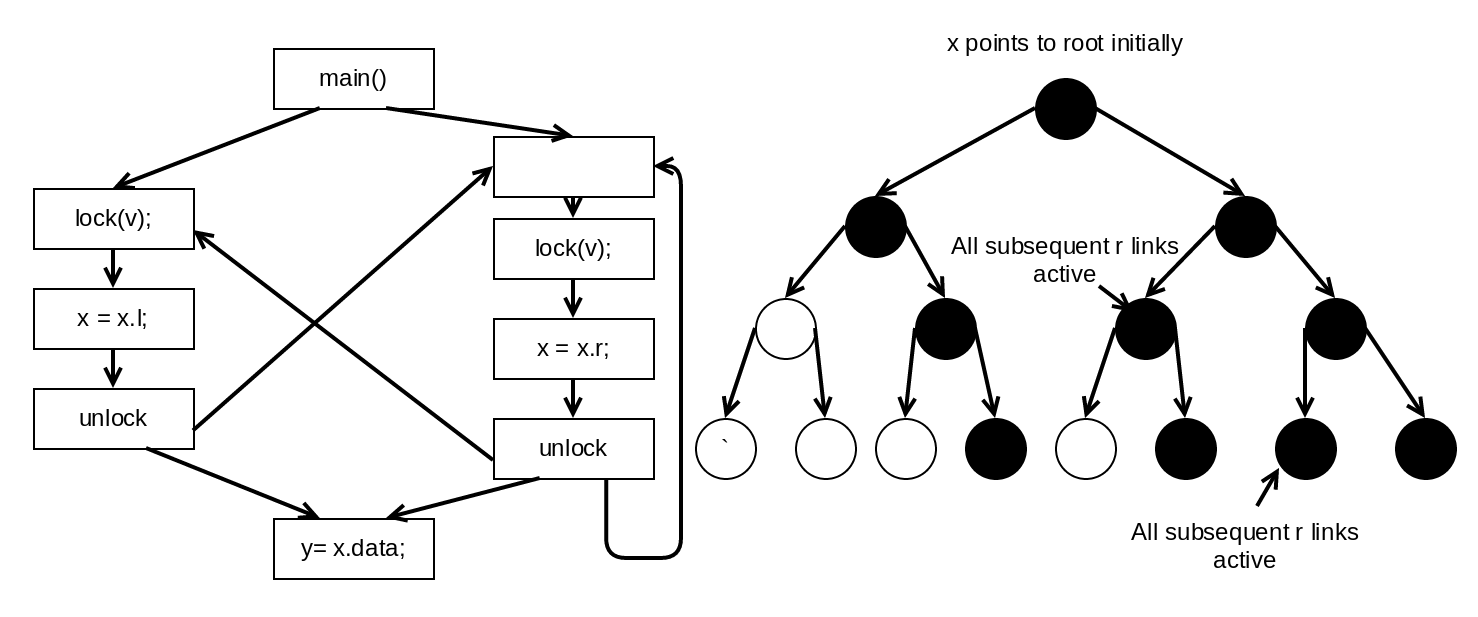
\includegraphics[width=0.8\textwidth]{Figures/tree3.png}
	\caption{Another Concurrent access example in a tree}
	\label{fig:ch5example}
\end{figure}

Another interesting example is the case when both the loops are outside critical sections in Figure 6.5. This will lead to any number of executions of $C_1$ and $C_2$ and interleaving are also possible. Thus the access graph expected for this kind of execution is \emph{x.\{l\textsuperscript{*}.r\textsuperscript{*}\}\textsuperscript{*}} . Starting with $C_1$, either multiple executions of $C_1$ and $C_2$ are possible. Also there is no restriction on the thread switchings. So for this example, all the nodes of the tree can be live/accessed. \\

\begin{figure}
	\centering
	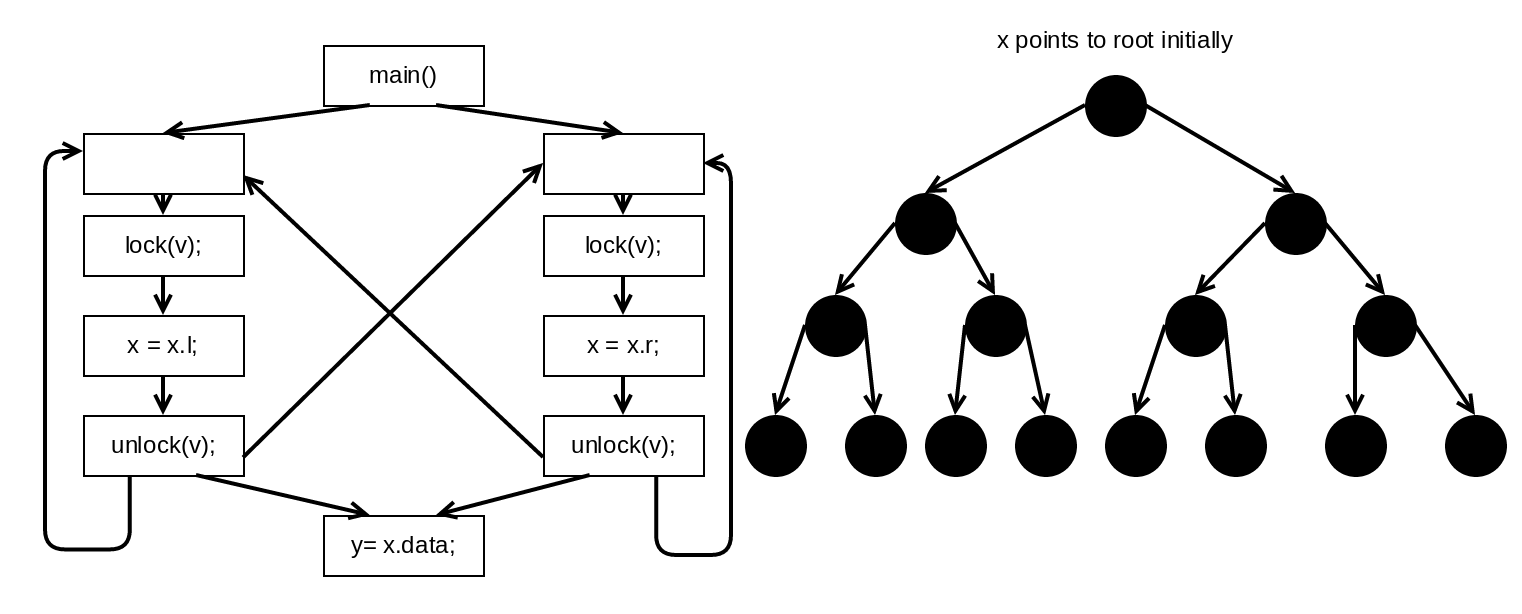
\includegraphics[width=0.8\textwidth]{Figures/tree4.png}
	\caption{Another Concurrent access example in a tree}
	\label{fig:ch5example}
 
\end{figure}

From all these examples, we can think of a way to propagate data flow values/access graphs across the synchronized control flow graph. We would have $n$ starting points , where $n$ is the number of threads in the program. Starting from a thread, data flow values are propagated along valid execution sequences. A valid execution sequence is such that all the thread switchings are consistent. This is ensured by examining all the critical sections. In a valid execution sequence, critical sections with no loops outside it appear only once. \\

For instance, in Figure 6.2 execution sequences possible are $T_1$,$T_2$ or $T_2$,$T_1$. We can also write this in terms of execution over critical sections. For this we will first need to run an analysis on each thread locally and find out the critical section(s) present. After identification, we also need to figure out whether the critical sections can be executed once or any number of times. Once we have the results from the intra-thread analysis, we will add the inter-thread edges to generate execution sequence over critical sections. For figure 6.2 and 6.3 the execution sequence can be either $C_1$,$C_2$ or $C_2$,$C_1$ since $count_c1$ and $count_c2$ is exactly 1. While in case of Figure 6.4, the possible executions are $C_1$,$C_2$\textsuperscript{*} and $C_2$,$C_1$,$C_2$\textsuperscript{*}. Only $count_c1$ is exactly 1.  \\

Consider an example for the above in Figure 6.6. Critical section of Thread 1 has 2 statements and that of Thread 2 has loop around the critical section. Nodes $C_1$ and $C_2$ are denoting these critical sections. $C_2$ has an edge from unto itself, denoting that it can be executed any number of times. Edges from $C_1$ to $C_2$ and from $C_2$ to $C_1$ are inter-thread edges. $count_c1$ is exactly equal to one. Let us start the analysis from thread 1. Possible execution path is $C_1$,$C_2$\textsuperscript{*}. We are considering heap liveness analysis, which is a backward analysis. Starting data flow analysis from thread 1, $C_1$, we get the access graph \emph{x.l.r} at the start of $C_1$. Transferring this graph to $C_2$, we obtain the access graph \emph{x.l2\textsuperscript{*}.l1.r}. Suppose we start from Thread 2. The execution path is $C_2$\textsuperscript{+},$C_1$,$C_2$\textsuperscript{*}. So the access graph obtained after the first step ($C_2$\textsuperscript{+}) is \emph{x.$l_2$\textsuperscript{+}}. After the second step ($C_2$\textsuperscript{+},$C_1$), we obtain \emph{x.$l_1$.$r_1$.$l_2$\textsuperscript{+}}. And finally upon transferring the value to $C_2$ again we obtain, \emph{x.$l_2$\textsuperscript{+}.$l_1$.$r_1$.$l_2$\textsuperscript{+}}. Note that, we do not merge the two $l_2$ nodes . This ensures that the access graph obtained will be such that, critical section $C_1$ will be executed only once. We have found a way to ensure this condition by not merging two nodes of the thread, if there is a thread switch to a thread whose critical section can only be executed once.

\section{Representation for execution sequences}

In the previous section, we had discussed about performing analysis along the possible execution sequences. It would ensure that the synchronized inter-thread edges do not simply act as loops. Also, merging along inter-thread execution paths was not allowed. We would store information in the graph to distinguish between inter \& intra thread edges. Our aim is to build an automata-like representation of thread switches, actually critical section executions. Before doing that we would need to perform forward/backward analysis in each thread and generate the intra-thread execution sequence. This will be sequential. Using this information, an inter thread automata would be built, whose current state represents a program execution upto that point. finally we would generate access graphs for each path in the inter-thread automata. \\

The following is a description of the procedure to generate the inter-thread automata. First generate an automata of critical sections for each thread. (This is the intra-thread step). In addition to this, identify for all critical sections if they are executed only once or any number of times. For each critical section, connect all the critical sections of all other threads. This is the inter-thread edge. This needs to be triggered upon a condition. In addition to this, for each critical section a counter storing the number of times the critical section is visited/executed is stored. The condition for an intra-thread edge entering a critical section $C_i$ is based on the counter for $C_i$ being strictly less than 1 if $C_i$ can only be executed once. Otherwise, there is no need for a condition on inter-thread edges. \\

The above construction would lead to formation of a transition system. See figure 6.7 for an example 6.2. $C_1$ and $C_2$
are critical sections of thread 1 and 2 respectively. Since both of them can only be executed once, the incoming edge on $C_i$ is triggered by the condition that count-ci \textless 1. \\

Note that conditions on edges will only be of this form. We may have conjunction and disjunction over multiple conditions for an edge. Let us take the same example of figure 6.6. Since all the edge predicates/conditions are of the type $var_i$ \textless 1, we can try to convert this transition system to an automata. This basically some states of the automata need to be visited only once. This can be ensured by removing that state from the automata, and generating 2 copies of the remaining xautomata. All incoming edges to state $S_i$ are connected from states in $copy_1$ and all the outgoing edges from $S_i$ are connected to nodes in $copy_2$. the starting state is the starting state of $copy_1$. All other non-reachable states in $copy_2$ should be removed. Note that this results in duplication of some states. Say we have $S_j$ and $S_j'$ and we have removed $S_i$ from the automata. Suppose in the original automata the condition for incoming edges into $S_j$ was $C_j$ \textless 1. Upon duplication we would need to ensure the condition on $S_j'$ would be $C_j$ \textless 1 \&\& $C_j'$ \textless 1. Figure 6.7 shows the schematic of the step we have just described. Also note that edges outgoing from S to $S_j'$ having the condition $C_j'$ \textless 1 will be ANDed with the condition of $S_j$, where $S_j'$ is the duplicate of $S_j$ in the right copy of A minus \{S\}. Alos note that the left copy satisfies the invariant $C_S$ = 0 and the right side satisfies the invariant $C_S$ >= 1. These predicates can be used to convert dotted edges to either solid edges (without conditions) or no edges (if the invariant makes the predicate false). Sometimes, it can simply set an argument of a conjunction condition to true and simplify the condition. See figure 6.8 for the conversion to automata of figure 6.6. we will obtain the execution sequences. And then we will perform analysis for along all these thread contexts. And also note that we will not merge across inter-thread edges.  Similarly we can convert other examples in chapter 5 to this form, by this method. \\
   
Note that this method of propagation of data flow values along valid thread contexts can be applied to any analysis, not just heap liveness analysis.  

\begin{figure}
	\centering
	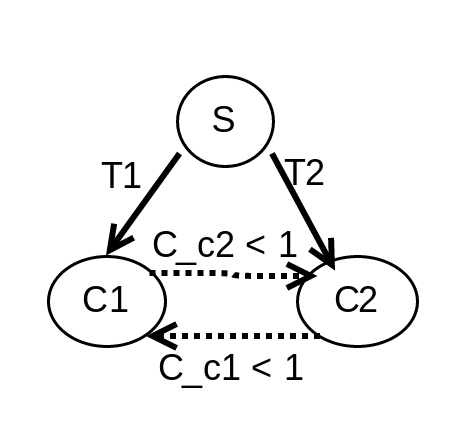
\includegraphics[width=0.4\textwidth]{Figures/automata_rep.png}
	\caption{An example transition system}
	\label{fig:ch5example}
\end{figure}


\begin{figure}
	\centering
	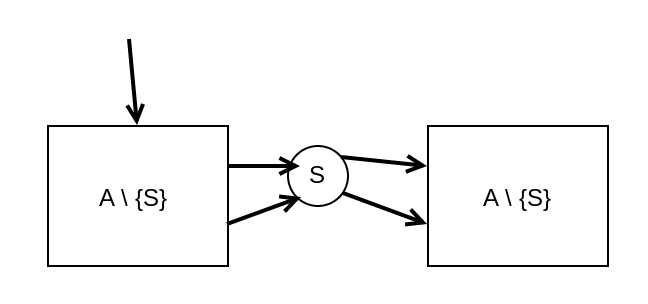
\includegraphics[width=0.8\textwidth]{Figures/automata_state.png}
	\caption{Ensuring S gets visited only once for a valid path}
	\label{fig:ch5example}
\end{figure}


\begin{figure}
	\centering
	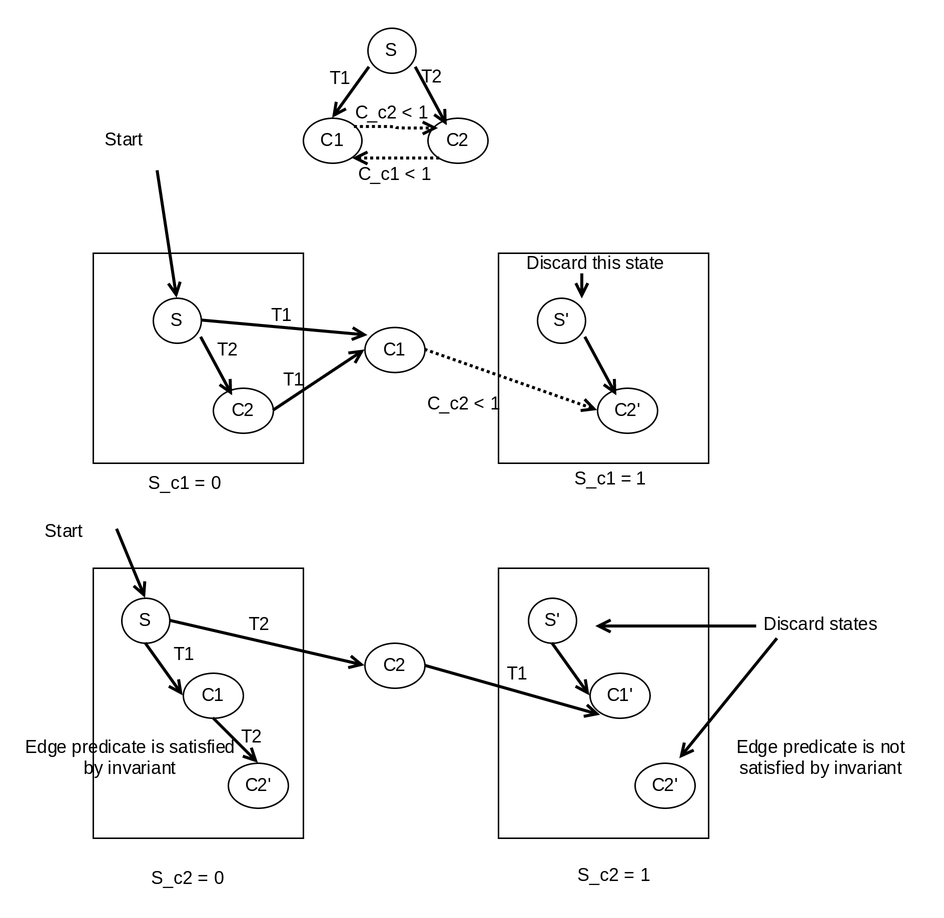
\includegraphics[width=0.8\textwidth]{Figures/automata_conv.png}
	\caption{Converting the condtion based transition system to automata like structure.}
	\label{fig:ch5example}
\end{figure}